%!TEX root = stability_manifold_TSP.tex


%%%%%%%%%%%%%%%%%%%%%%%%%%%%%%%%%%%%%%%%%%%%%%%%
%%%%%%%%%%%%%%%%%% FIGURE %%%%%%%%%%%%%%%%%%%%%% 
%%%%%%%%%%%%%%%%%%%%%%%%%%%%%%%%%%%%%%%%%%%%%%%%
\begin{figure*}[h]
\centering
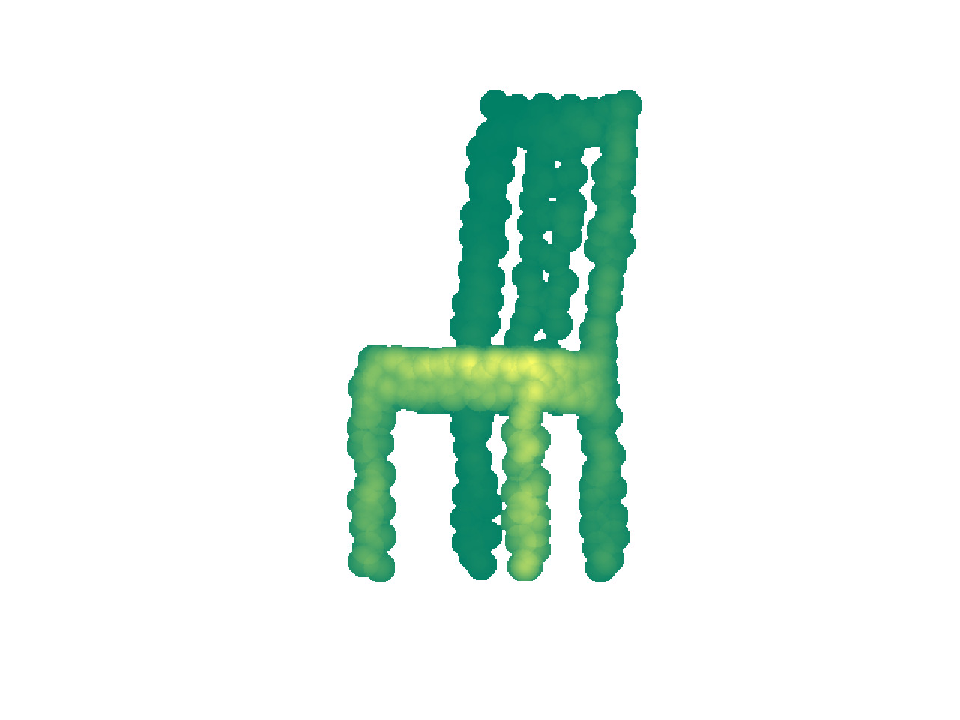
\includegraphics[trim=130 0 80 0,clip,width=0.15\textwidth]{chair_large-eps-converted-to.pdf}
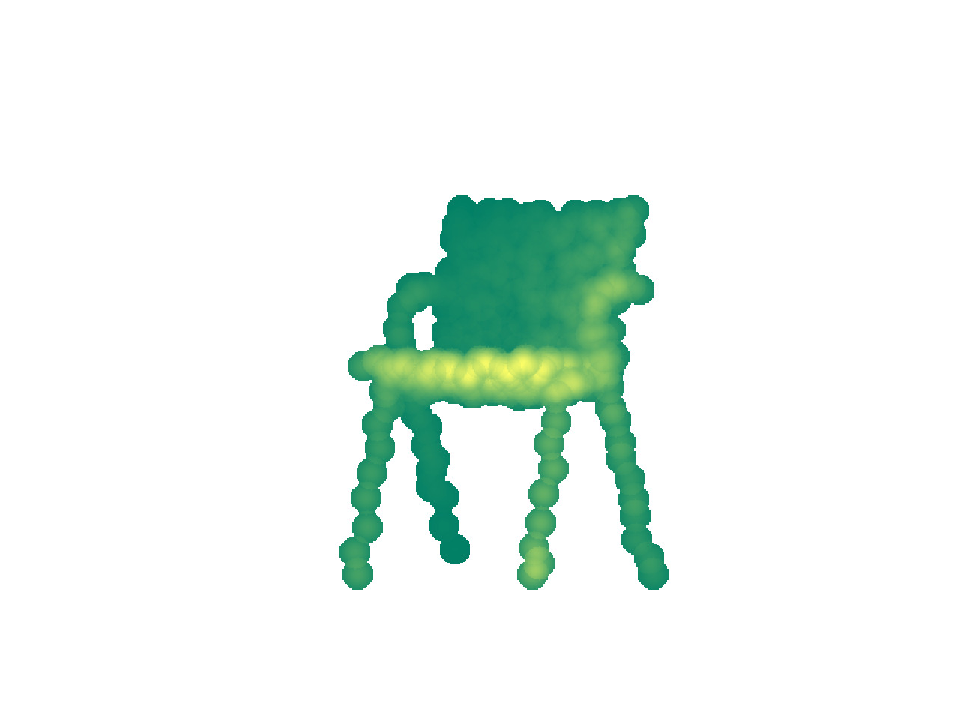
\includegraphics[trim=90 0 100 0,width=0.15\textwidth]{chair_large1-eps-converted-to.pdf}  
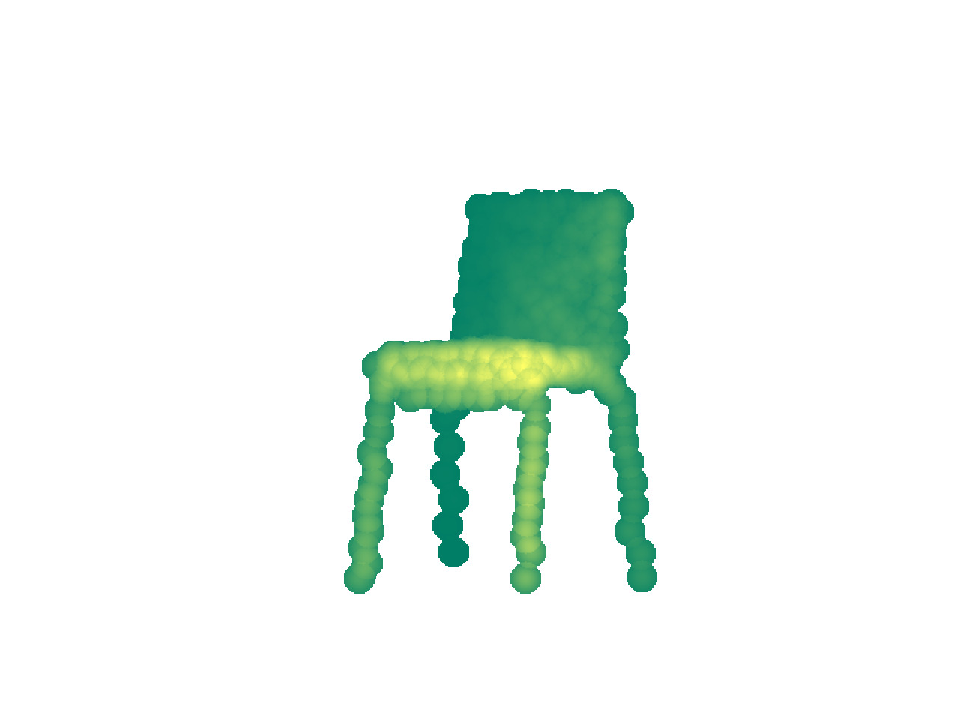
\includegraphics[trim=60 0 100 0,width=0.15\textwidth]{chair_large2-eps-converted-to.pdf} 
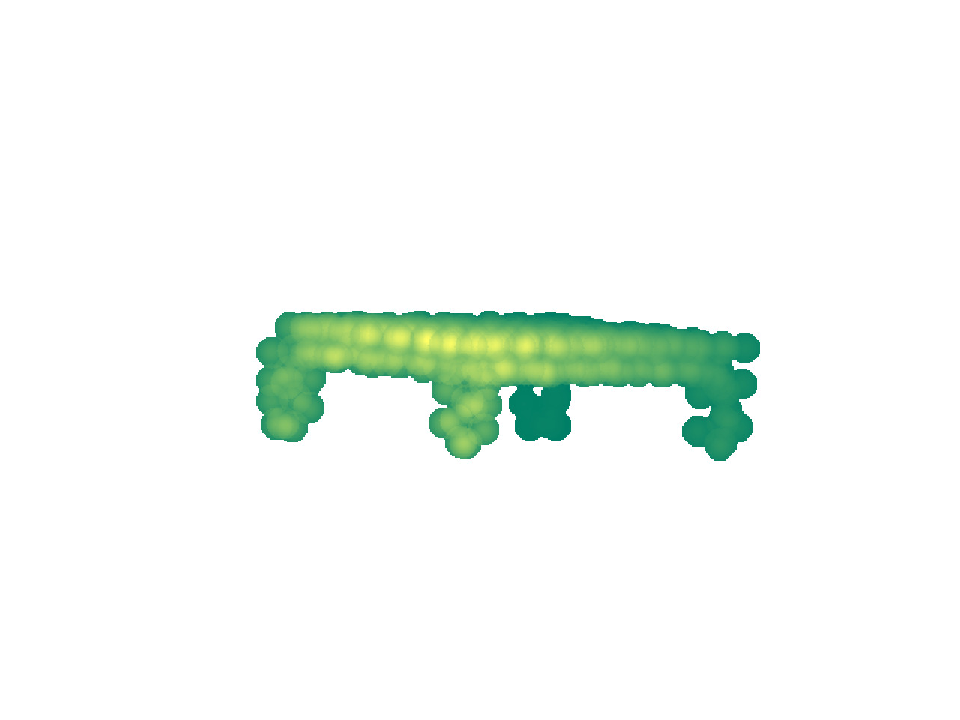
\includegraphics[trim=60 0 50 0,width=0.15\textwidth]{table_large-eps-converted-to.pdf}  
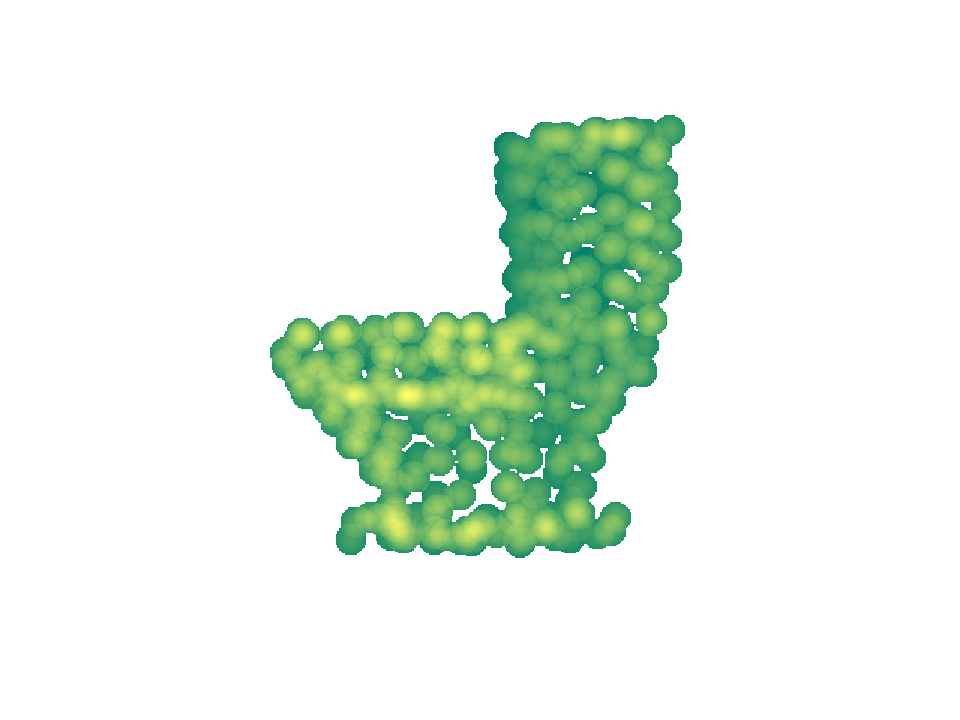
\includegraphics[trim=60 0 100 0,width=0.15\textwidth]{toilet_large-eps-converted-to.pdf}  
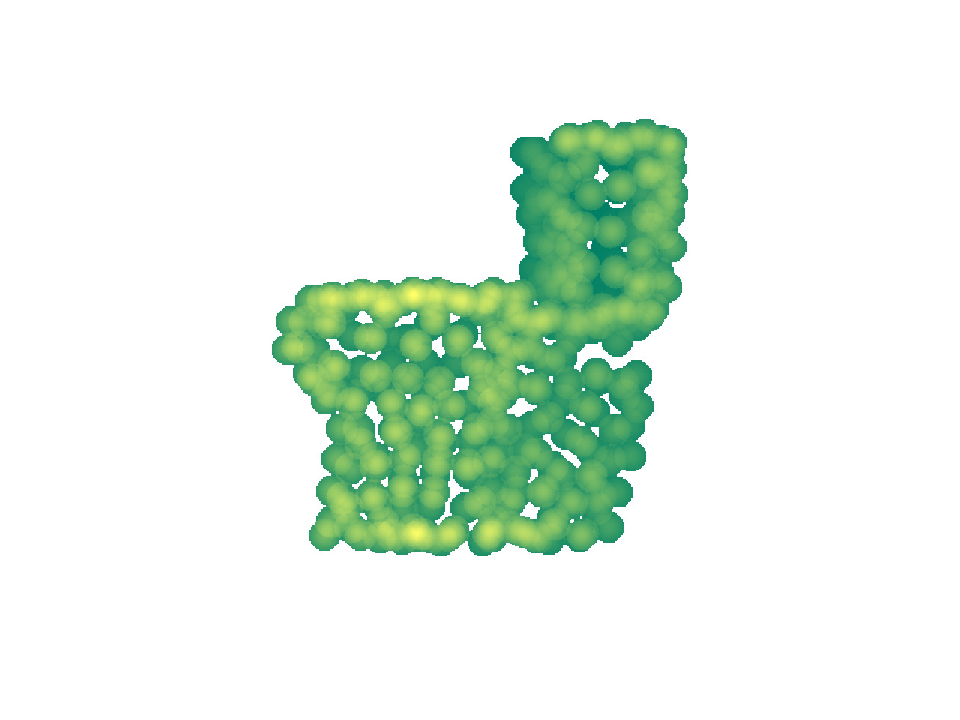
\includegraphics[trim=60 0 100 0,width=0.15\textwidth]{toilet_large1-eps-converted-to.pdf} 

\caption{Point cloud models with 300 sampling points in each model. Our goal is to identify chair models from other models such as toilet and table. }
\label{fig:points}
\end{figure*}

\myparagraph{Dataset} We evaluate our MNN stability results on the ModelNet10 \cite{wu20153d} classification problem. The dataset contains 3991 meshed CAD models from 10 categories for training and 908 models for testing. For each model, 300 points are uniformly randomly sampled from all points of the model to form the point cloud. Each point is characterized by the 3D coordinates as features. We formulate the problem by modeling a dense graph neural network model to approximate MNN. Each node in the graph can be modeled as the sampling point and each edge weight is constructed based on the distance between each pair of nodes.  In this work our goal is to identify the CAD model for chairs as is illustrated in Figure \ref{fig:points} with the models for chair labeled as 1 and the others as 0. We deform the underlying manifold structure by adding random perturbations to the coordinates of the sampling points. By comparing the differences of the classification error rates, we aim to show that MNNs with Lipschitz continuous and integral Lipschitz continuous manifold filters are stable via looking into the performance of the approximated GNNs. 

\myparagraph{Neural network architectures} We build dense graphs to approximate the point cloud models. We use the coordinates of each point as node features. By connecting a point with all the other points in the point cloud, the edge weight is defined based the distance between every two points and a Gaussian kernel. The Laplacian matrix is calculated for each input point cloud model. We implement different architectures, including Graph Filters (GF) and Graph Neural Networks (GNN) with 1 and 2 layers,  to solve the classification problem. The architectures with a single layer contain $F_0=3$ input features which are the 3d coordinates of each point, $F_1=64$ output features and $K=5$ filter taps. While the architectures with 2 layers has another layer with $F_2= 32$ features and $5$ filter taps. We use the ReLU as nonlinearity. The learned graph filters are not regularized in architectures with 'NoPel' while graph filters in the other architectures are both Lipschitz and integral Lipschitz. All architectures also include a linear readout layer mapping the final output features to a binary scalar that estimates the classification. 

\myparagraph{Discriminability experiment} We train all the architectures with an ADAM optimizer \cite{kingma2014adam} with learning rate set as 0.005 and decaying factors as 0.9, 0.999 by minimizing the entropy loss. The training point cloud models are divided in batches of 10 over 40 epochs. We run 5 random point samplings for all the architectures and we show the average classification error rates across these realizations as well as the standard deviation in Table \ref{tb:results}. We can observe that with the use of non-linearity, Graph Neural Networks perform better compared with Graph Filters. Architectures with more layers learn more accurate models which also leads to better performances.  

%%%%%%%%%%%%%%%%%%%%%%%%%%%%%%%%%%%%%%%%%%%%%%%%
%%%%%%%%%%%%%%%%%% TABLE %%%%%%%%%%%%%%%%%%%%%%% 
%%%%%%%%%%%%%%%%%%%%%%%%%%%%%%%%%%%%%%%%%%%%%%%%
\begin{table}[h]
\centering
\begin{tabular}{l|c} \hline
Architecture    & error rates   \\ \hline
GNN1Ly	& $8.04 \% \pm 0.88\% $   \\ \hline
GNN2Ly		& $4.30\% \pm 2.64\%$   \\ \hline
GF1Ly		& $13.77\% \pm 6.87\%$   \\ \hline
GF2Ly	& $12.22\% \pm 7.89\%$   \\ \hline
\end{tabular}
\caption{Classification error rates for model 'chair' in the test dataset. Average over 5 data realizations. The number of nodes is $N=300$.}
\label{tb:results}
\vspace{-3mm}
\end{table} 

\myparagraph{Stability experiment} We test the same trained Graph Neural Networks and Graph Filters with 2 layers on perturbed test point cloud models with different perturbation levels. We perturb the test point clouds by adding a Gaussian random variable with mean $\epsilon$ and variance $2\epsilon$ to each coordinate of every sampling point, which can be seen as a deformation of the underlying manifold. We measure the stability by computing the difference between the error rates achieved based on the original test point cloud models and the perturbed ones. In Figure \ref{fig:sim}, we see that this difference increases when the perturbations become larger, but overall the differences are small. We also observe that Graph Neural Network is more stable compared with Graph Filters. Furthermore, the Graph Neural Networks and Graph Filters with Lipschitz continuous and integral Lipschitz continuous filters are more stable. Both of these observations validate our stability results. 

%%%%%%%%%%%%%%%%%%%%%%%%%%%%%%%%%%%%%%%%%%%%%%%%
%%%%%%%%%%%%%%%%%% FIGURE %%%%%%%%%%%%%%%%%%%%%% 
%%%%%%%%%%%%%%%%%%%%%%%%%%%%%%%%%%%%%%%%%%%%%%%%
\begin{figure}[h]
  \centering
  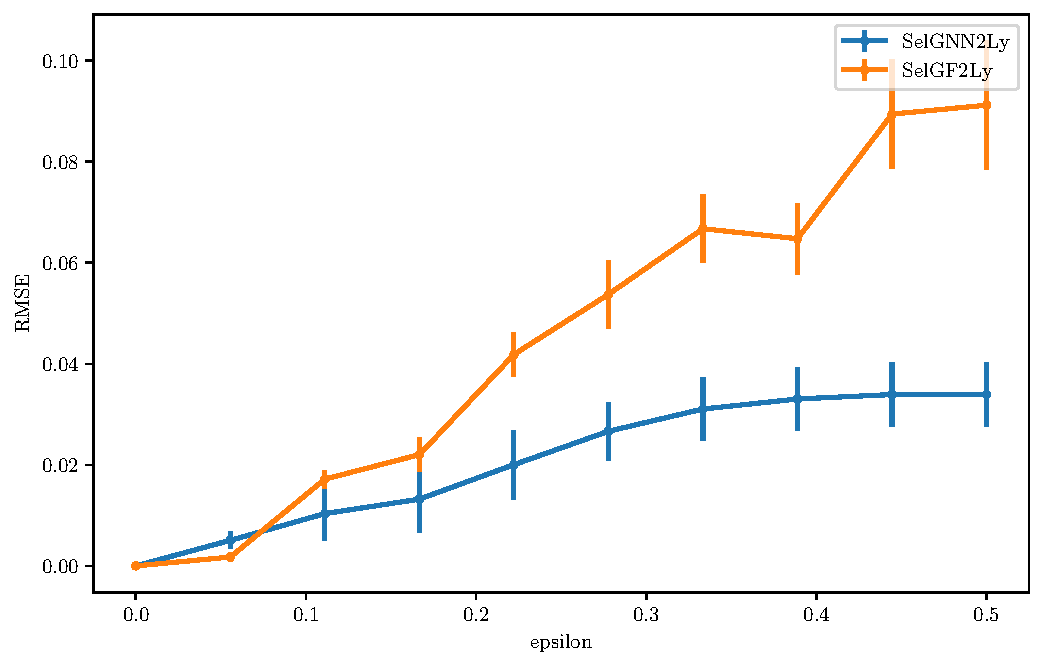
\includegraphics[height=4.5cm,width=6.5cm]{allCostTest.pdf}
\caption{Difference between error rates on the original test dataset and the deformed one. }
\label{fig:sim}
\end{figure}

%%%%%%%%%%%%%%%%%%%%%%%%%%%%%%%%%%%%%%%%%%%%%%%%
%%%%%%%%%%%%%%%%%% FIGURE %%%%%%%%%%%%%%%%%%%%%% 
%%%%%%%%%%%%%%%%%%%%%%%%%%%%%%%%%%%%%%%%%%%%%%%%
\begin{figure}[h]
  \centering
  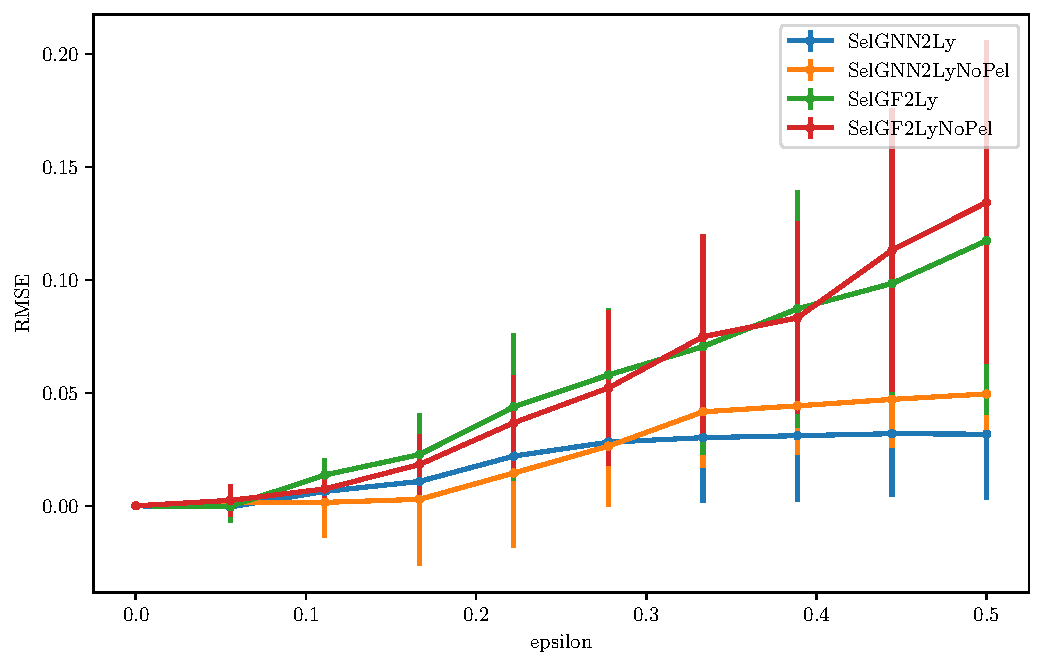
\includegraphics[height=4.5cm,width=6.5cm]{allCostTest_nopenalty.pdf}
\caption{Difference between error rates on the original test dataset and the deformed one. }
\label{fig:sim}
\end{figure}
To further verify the discriminability under perturbations, we trained and tested the architectures with perturbed dataset. We can see from Table \ref{tb:results-perturb} that both GNN and GF can identify the chair model with small error rates while the error rates grow slightly with the increase of perturbation levels. GNNs still outperform GFs in discriminablity with the help of nonlinearity.

%%%%%%%%%%%%%%%%%%%%%%%%%%%%%%%%%%%%%%%%%%%%%%%%
%%%%%%%%%%%%%%%%%% TABLE &&&&&%%%%%%%%%%%%%%%%%% 
%%%%%%%%%%%%%%%%%%%%%%%%%%%%%%%%%%%%%%%%%%%%%%%%
\begin{table}[h]
\centering
\begin{tabular}{l|c |c  } \hline
Architecture    & $\epsilon = 0.2$ & 0.4   \\ \hline
GNN2Ly		& $7.37\% \pm 1.43\%$ &  $7.71\% \pm 3.96\%$ \\\hline
GF2Ly	& $13.76\% \pm 6.82\%$  & $13.54\% \pm 7.16\%$  \\ \hline\hline
Architecture    & $\epsilon = 0.6$ & 0.8   \\ \hline
GNN2Ly& $8.04\% \pm 2.83\%$ & $11.01\% \pm 6.33\%$  \\ \hline
GF2Ly	& $14.76\% \pm 5.67\%$ & $16.04\% \pm 6.34\%$ \\ \hline
\end{tabular}
\caption{Classification error rates for model 'chair' with perturbed training and test dataset. Average over 5 data realizations. The number of nodes is $N=300$.}
\label{tb:results-perturb}
\vspace{-3mm}
\end{table} 

% We take GNNs as discretizations of MNNs to help verify our results. By constructing a graph model to represent the wireless adhoc network structure, we can solve the optimal resource allocation problem with a GNN. We consider a wireless adhoc network with $n=50$ pairs of transmitters and receivers within a range of $[-50m, 50m]^2$, i.e., the transmitter density is $\rho=0.02 \text{ transmitter}/m^2$. The receiver $r(i)$ is paired with the transmitter $i$ by dropping randomly around the transmitter. The channel link state between each transmitter and receiver is denoted  $[\bbS(t)]_{ij}:=s_{ij}(t)\in\reals_+$ at time $t$ between transmitter $i$ and receiver $r(j)$. %We measure the link condition by combining the large-scale pathloss gain and a random fast fading gain, which can be written as: $h_{ij}=\log(d_{ij}^{-2.2} h^f)$. The distance between transmitter $i$ and receiver $r(j)$ is denoted as $d_{ij}$ while $h^f\sim \text{Rayleigh}(2)$ stands for the fast fading gain. 
% Here, we focus on the power allocation problem among $n$ transmitters over an AWGN channel with interference, with $\bbp(\bbS)=[p_1(\bbS),p_2(\bbS),\hdots,p_n(\bbS)]$ denoting the power allocated to each transmitter under channel condition $\bbS$. The Shannon channel rate of transmitter $i$ is represented as $f_i$. The goal is to maximize the sum rate capacity under a total power budget $P_{max}$. The problem can be formulated as an optimization problem as
% \begin{align}
% %\label{eqn:prob_sim}
% f^* &=\max_{\bbp(\bbS)} \sum_{i=1}^n f_i \\
% s.t.\quad \nonumber &r_i=\mathbb{E}\left[  \log\left(1+\frac{s_{ii}^2 p_i(\bbS)}{1+ \sum\limits_{j\neq i}s_{ij}^2 p_j(\bbS)}\right) \right],\\
%   \nonumber & \mathbb{E}[\bm{1}^T\bbp]\leq P_{max},\quad p_i(\bbS)\in \{0,p_0\}.
% \end{align}
% With the transmitters and receivers modeled as graph nodes, the links between each transmitter and receiver can therefore be seen as edges. The channel matrix $\bbS$ composed of link conditions can be seen as the graph shift operator. 
% In the real world, the distribution of the transmitters can vary, which can be seen as a deformation to the underlying manifold. To capture this, we model the deformation by changing the density and the location distribution of the transmitters respectively. 

%  We measure policy performance in terms of the ratio of the sum-of-rate achieved by the GNN and a baseline heuristic method (WMMSE \cite{shi2011iteratively}) after training for 40,000 iterations (details on hyperparameters and other settings can be found in the appendices). We observe that the sum of capacity converges and the trained GNN can achieve the optimal power allocation policy on the original graph. By employing the same GNN (i.e., with the same parameters) on the deformed graph, we measure stability by computing the difference between the ratios achieved in the original wireless network setting and in the deformed settings described in the caption of Figure \ref{fig:sim}. In this figure, we see that this difference increases when the perturbations become larger, but overall the differences are small. We also compare GNNs with different architectures, and observe that deeper and wider GNNs are less stable. Both of these observations validate our stability results.

% \begin{figure}[t]
%   \centering
%   \subfloat[Stability to varying density. \label{fig:a}]{\includegraphics[height=4.5cm,width=6.5cm]{densityratio.eps}}\qquad
%   \subfloat[Stability to mixed uniform distributions. \label{fig:b}]{\includegraphics[height=4.5cm,width=6.5cm]{mixeduniformratio.eps}}
% \caption{Difference between the sum-of-rate ratios on the original wireless network setting and the deformed one. The $x$ axis in Figure \ref{fig:a} stands for the change on transmitter density, i.e., the perturbed density is given by $\rho'=\rho/(1-\sigma_1)$. In Figure \ref{fig:b}, the $x$-axis measures the perturbation to the original uniform distribution of the transmitters' locations. In the range $[-50m,0]$, a transmitter is dropped with probability $(1+\sigma_2)/2$, and in $[0, 50m]$, with probability $(1-\sigma_2)/2$ on each direction.}
% \label{fig:sim}
% \end{figure}